% ==========================================
% 第一篇 导入过场页
% ==========================================
\cleardoublepage
\thispagestyle{empty} % 让过场页干干净净，没有页眉页脚

\vspace*{6cm} % 整体垂直向下偏移，营造留白的高级感

\begin{center}
	% 篇章标题
	{\heiti\erhao 第一篇\quad 我们经历了什么} 
	\addcontentsline{toc}{part}{第一篇\quad 我们经历了什么}
	
	\vspace{2cm} % 标题与文案之间的间距
	
	% 灵魂文案
	{\songti\xiaosi \textit{一个1994年的加密算法，至今还守护着中国80\%的大门。\\ [0.5em]一场即将到来的量子风暴，将让包括其替代者在内的一切经典密码体系土崩瓦解。\\ [0.5em]真正危险的地方，不是“门禁不够先进”，而是很多门禁系统看起来还在正常工作，\textbf{但安全性其实早就透支了}。}}
\end{center}

\vfill
\cleardoublepage % 过场页结束，下一页正式开始第三章正文

% ==========================================
% 第一章
% ==========================================
\chapter{一扇守不住的门——中国门禁卡安全现状}

\section{一个价值百亿的市场，建立在纸糊的安全之上}

门禁不是小生意，而是城市更新、社区治理、校园管理、园区安防、酒店运营每天都在用的底层基础设施。\textbf{2022年，中国门禁卡机市场规模已达41.96亿元}；2024年，国内IC卡行业市场规模预计\textbf{突破140亿元}，同年智慧门禁系统市场规模达到\textbf{236亿元}（年复合增长率达12.16\%），\textbf{2025年，全球门禁市场更将突破400亿美元}。

从市场分布来看，\textbf{住宅细分市场占比高达40.08\%}，是门禁读卡器领域占比最高的应用场景。也就是说，国内绝大多数居民家门口的门禁，都处于这个市场的覆盖范围内。行业主流技术路线沿着 ID卡 $\rightarrow$ M1卡 $\rightarrow$ MIFARE Plus/DESFire $\rightarrow$ CPU卡迭代，而目前国内门禁市场的绝对主力，\textbf{仍是1994年正式发布的M1卡}。

仅2024年，全国就计划新开工改造城镇老旧小区5.4万个；智慧社区与平安城市建设\textbf{年投资超2000亿元}，老旧小区安防改造催生百亿级市场。这说明门禁不会退出舞台，只会越来越深地嵌入各种高价值场景。

行业格局上，国内市场以海康威视、大华股份为龙头，国际市场则被 ASSA ABLOY、Honeywell 等巨头把控。但截至目前，上述国内外头部企业的主流商用产品，\textbf{均未在门禁核心加密层实现可规模化落地的量子安全级突破}。

\textbf{行业拐点信号：}Connectivity Standards Alliance（连接标准联盟，简称CSA）已于2026年全球正式发布 \textbf{Aliro 1.0规范}，并获得Apple、Google、Samsung等移动钱包生态支持。这个信号非常明确：\textbf{下一代门禁的竞争，不再只是“能不能开门”，而是“能不能既安全，又互通，还能长期演进”。}

\section{M1卡：一个1994年的“定时炸弹”}

M1卡的问题，不是“可能有风险”，而是已经被厂商、研究界和现实事件\textbf{反复证实的不安全}。它是1994年由NXP发布的产品，核心的 Crypto-1 算法仅配备了 \textbf{48bit 密钥}。这套诞生于30年前的技术，早在2008年就被逆向工程全面破解，\textbf{在2015年核心算法被完全攻破}，同年NXP官方已宣布不再推荐使用，但至今\textbf{仍占据中国IC门禁卡市场约80\%的份额}。

目前，已有多种M1卡的破解方式被证实，且每一种都有成熟的落地手段：
\begin{enumerate}
	\item \textbf{暴力破解：}M1卡本身无法记录密码错误次数，永远不会被锁定，可被无限次暴力破解。
	\item \textbf{嵌套认证攻击：}只要知道一个扇区的密钥，就能通过嵌套认证攻击破解整张卡的全部加密内容。
	\item \textbf{Darkside攻击：}即便在零密钥条件下，也能通过Darkside攻击完成对全加密卡的破解。
	\item \textbf{重放攻击：}PRNG算法存在的致命缺陷让随机数序列可被预测，攻击者可通过重放攻击直接复刻合法权限。
	\item \textbf{嗅探攻击：}只要窃听一次合法的刷卡通信，就能通过嗅探攻击推算出完整密钥。
	\item \textbf{硬件后门转储：}2024年最新曝光的复旦芯片甚至存在硬件后门，\textbf{能在5分钟内完成全加密卡的完整数据转储，完全无解}。
\end{enumerate}

更可怕的是\textbf{极低的作恶门槛}：30元的PN532模块、开源免费的破解软件、一部安卓手机。哪怕是完全不懂技术的小白，跟着网上的教程视频，半小时就能完成全流程破解；街边的配锁店，\textbf{5秒钟就能复刻一张完全可用的门禁卡}。

\section{真实犯罪案例与社会影响}

\textbf{案例一：未成年人利用M1卡漏洞盗刷校园一卡通}

广西贺州八步区法院公开审理的案件显示，5名未成年人利用网购的IC卡复制设备克隆校园IC卡，非法盗刷2万多元。警方实验证实：看完网购教程后，\textbf{不到半小时就能完成软件安装、原卡读取、复制和克隆}，复制出的饭卡、门禁卡均能正常使用。这起案子最扎心的地方，在于把低安全卡片变成“可复制钥匙”的门槛低到了令人发指的程度。

\begin{figure}[htbp]
	\centering
	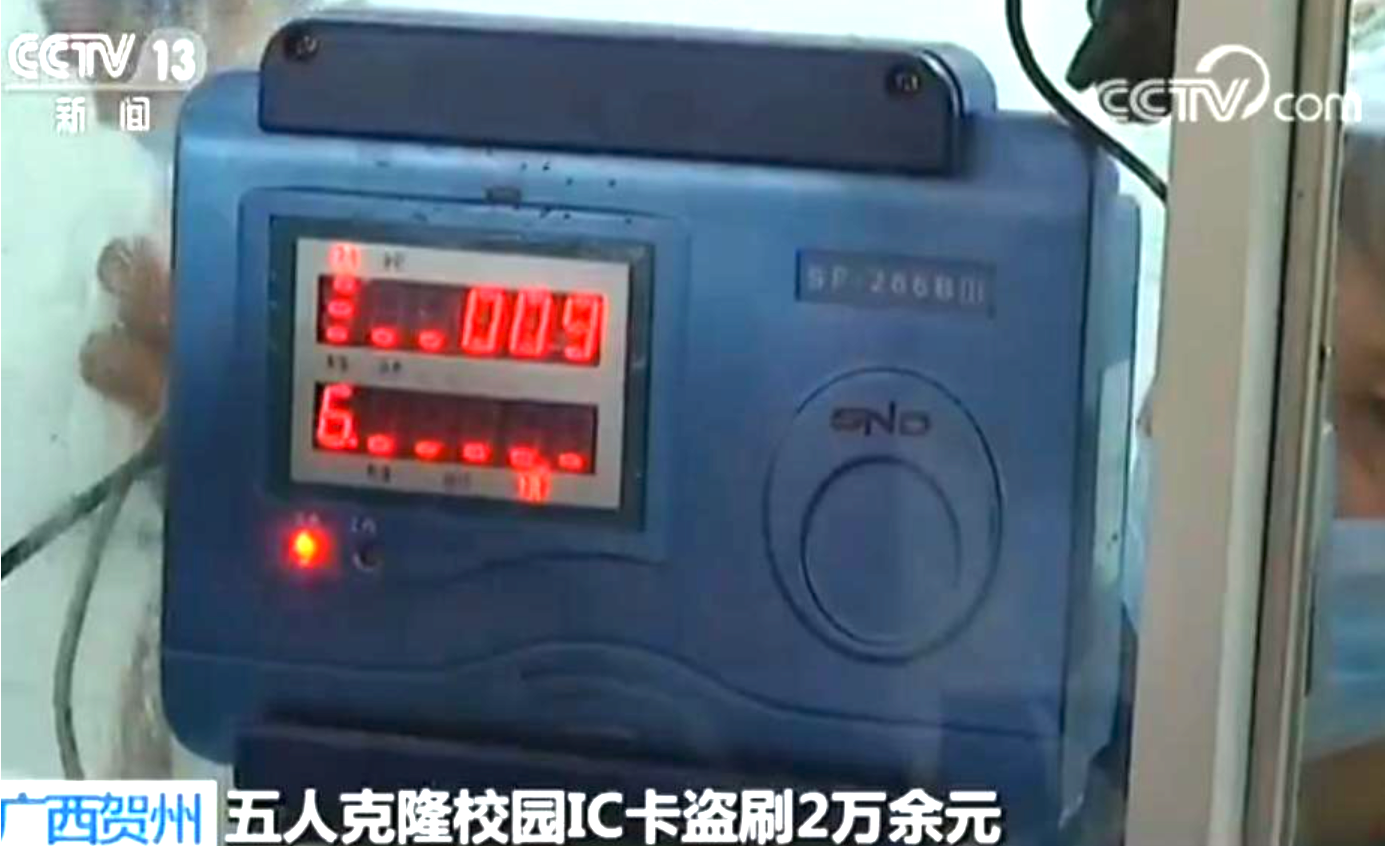
\includegraphics[width=0.75\textwidth]{figures/M1card.png}
	\caption{广西贺州未成年人克隆校园IC卡盗刷案新闻报道}
	\label{fig:case1_school}
\end{figure}

\textbf{案例二：全球酒店门锁“Unsaflok”漏洞}

dormakaba官方承认，Saflok系统存在与门卡底层数据保护相关的漏洞（CVE-2024-29916）：攻击者只要拿到任意一张有效或过期的房卡，就可能伪造门卡，打开该物业内的任意房门。这一漏洞\textbf{影响到131个国家超过1.3万处物业的300多万扇门}。

这两个典型案例一内一外构成完整链路：一旦门禁底层算法和凭证体系有结构性漏洞，影响就不再是一张卡、一个门，而可能是一整栋楼、一整家酒店，甚至\textbf{一个完整的物业系统}。

\section{M1卡的代价不是“便宜”，而是“昂贵”}

物业和开发商选择M1卡的唯一理由是“便宜”（单卡几毛钱）。但实际上，真正被忽视的是巨大的\textbf{后续成本（TCO）}：事故处置、系统补洞、运维返工、用户投诉以及最难修复的\textbf{信任损失}。门禁一旦被证明“可以复制”，它就沦为了一个迟早出事的摆设。

在法律层面，已有大量判例显示，因门禁卡漏洞导致业主失窃，\textbf{物业需承担20\%到50\%的赔偿责任}，单次赔偿达数万至十几万元。一个千户小区一次入室盗窃的赔偿金额，就已经远超全小区门禁卡升级的全部成本。看似省了几块钱，实则是赌上了业主的安全与物业的巨额赔偿。